\chapter{Experiments}
\label{ch.experiments}

% Neste capítulo
	This chapter evaluates the performance of Nanvix Microkernel Services for
	data exchange on \mppa, \ie \mailbox and \portal. The micro-benchmarks seek to
	stimulate different collective communication configurations that are common in a
	distributed system and present in the high-level services exported by Nanvix
	Multikernel. For instance, message exchange between servers and clients, work
	distribution, and collection of distribution results. Although the \sync service
	has no specific experiments, it was used in all benchmarks to synchronize all nodes
	before commencing communications.

% Como foram medidos os dados
	Micro-benchmarks measured the data volume and communication latency of each
	service through the \ioctl interface. In each cluster, only 1 \pe was used
	to run the application. This \pe requested microkernel services to perform
	communication. In \iocluster, only one of the available interfaces was used
	because of the necessity to use the interface associated with the logical ID
	of the node. The \iocluster also plays the master role when the communication
	routine requires a master-slave behavior.

% Quantas iterações, limitações de memória e desvio padrão
	\mppa has intrinsic characteristics that guarantee low variability between runs.
	Thus, 50 iterations of each benchmark were performed. The first ten iterations
	were discarded to eliminate the warm-up period. Finally, all results showed a
	standard error of less than 1\%.

	\section{Micro-benchmarks}

		To analyze the performance of the Communication Services, we used the typical
		routines for collective communication of \mpi and common behaviors between
		clients and servers. The following subsections conceptually introduced each
		of these routines and behaviors.

		\subsection{Broadcast}

			Broadcast is the most common technique among collective communication
			routines of the \mpi. In this routine, a node sends the same data to
			all existing nodes. This submission can be implemented in several ways,
			as such, flat tree, binary tree, double tree, and chain~\cite{mpi-survey}.
			\autoref{fig:exp-broadcast} presents the flat tree algorithm used in
			the benchmark. The flat tree defines that the root node should send
			data to everyone without delegating this function to other nodes.
			This routine can be used to send user inputs to a parallel program
			or to send configuration parameters to all nodes~\cite{url:mpitutorial}.

			\begin{figure}[!tb]
				\centering%
				\caption{Example of \mpi Broadcast}%
				\label{fig:exp-broadcast}%
				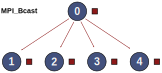
\includegraphics[width=.6\textwidth]{mpi-broadcast.pdf}%
				\fonte{Adapted from \citeonline{url:mpitutorial}.}%
			\end{figure}

		% \subsection{Scatter}

		% 	\begin{figure}[!tb]
		% 		\centering%
		% 		\caption{Example of \mpi Scatter}%
		% 		\label{fig:mpi-scatter}%
		% 		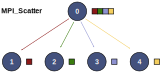
\includegraphics[width=.6\textwidth]{mpi-scatter.pdf}%
		% 		\fonte{Adapted from \citeonline{url:mpitutorial}.}%
		% 	\end{figure}

		% 	Resultados iguais ao do broadcast

		\subsection{Gather}

			Gather is the inverse operation of a broadcast variant called scatter.
			\autoref{fig:exp-gather} illustrates the reverse data flow, where this
			routine gathers the data distributed on a single node~\cite{url:mpitutorial}.
			Similarly to broadcast, a flat tree was implemented where all root
			nodes send their parts directly to the root node.

			\begin{figure}[!tb]
				\centering%
				\caption{Example of \mpi Gather}%
				\label{fig:exp-gather}%
				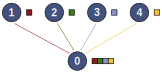
\includegraphics[width=.6\textwidth]{mpi-gather.pdf}%
				\fonte{Adapted from \citeonline{url:mpitutorial}.}%
			\end{figure}

		\subsection{AllGather}

			AllGather is a routine that does not have a root node, illustrated by
			\autoref{fig:exp-allgather}. As the name suggests, the routine performs
			several Gather operations so that all participating nodes end with all
			pieces of data gathered. Some possible algorithms are Ring Algorithm,
			Recursive Doubling, Gather followed by Broadcast Algorithm. The benchmark
			implements the Bruck Algorithm where each node will send its data to a node
			with distance $i$ and receive data from a distance $-i$ until all nodes
			contain the complete data.

			\begin{figure}[!tb]
				\centering%
				\caption{Example of \mpi AllGather}%
				\label{fig:exp-allgather}%
				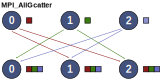
\includegraphics[width=.6\textwidth]{mpi-allgather.pdf}%
				\fonte{Adapted from \citeonline{url:mpitutorial}.}%
			\end{figure}

		\subsection{Ping-Pong}

			Ping-Pong is not an \mpi collective communication routine but represents
			communication from a server answering requests from client nodes.
			Ping-Pong illustrates communication by focusing on the master node,
			where the master receives and answers one request at a time.

			\begin{figure}[!tb]
			    \centering%
			    \caption{Example of Ping-Pong}%
			    \label{fig:exp-ping-pong}%
			    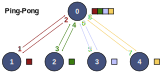
\includegraphics[width=.6\textwidth]{mpi-ping-pong.pdf}%
			    \fonte{Develop by the Author.}%
			\end{figure}

	\section{Portal Throughput Analysis}

		The first experiment sought to analyze the throughput provided by the
		Portal service. All micro-benchmarks involve 1 \iocluster and 16 \ccluters.
		\autoref{fig:exp-portal} shows the transfer rate in MB/s, varying the size
		of the buffer to be transmitted from 4~KB to 64~KB. They have not been
		tested with values ​​larger because of the memory limitation in the \ccluters.
		For instance, AllGather requires approximately a total space of 1~MB ($17 nodes \times 64 KB$).

		Results exhibit three distinct behaviors in the Portal results. First,
		the Broadcast was expected to have the worst transmission rate due to
		the use of a single data transmitter. Since the measurement was done
		on the receiver side, the last slave had to wait for master transmits
		to all other nodes, considerably reducing the transfer rate in the
		Broadcast. Second, the Gather and Ping-Pong routines showed similar
		results. This similarity is because the master node receives multiple
		requests and handles them serially one by one. The master node
		dictated the data flow in both benchmarks because transfer through
		the Portal is only performed when allowed by the receiver. Finally,
		the AllGather routine exhibited the best results because of the
		parallelism of communications. Also, each communication pair co-occur,
		and multiple read/write requests not happen int the same time on a node,
		softening the interruption of the master core. Overall, the results
		were as expected, but we believe that the use of \dma accelerators could
		significantly improve Portal performance.

		\begin{figure}[!tb]
			\centering%
			\caption{Throughput of the Portal.}%
			\label{fig:exp-portal}%
			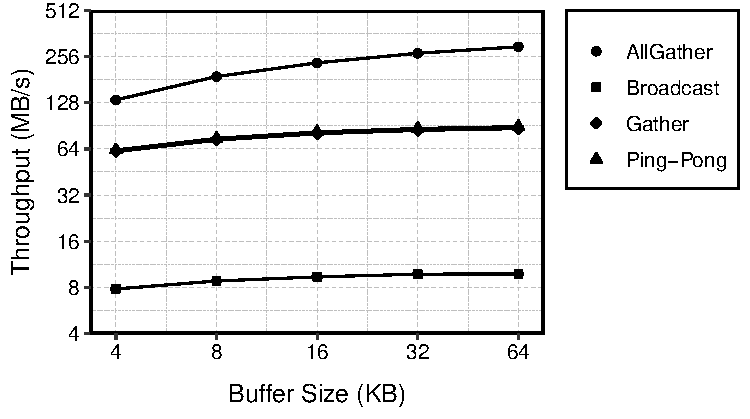
\includegraphics[width=.7\textwidth]{portal-throughput.pdf}%
			\fonte{Develop by the Author.}%
		\end{figure}

	\section{Mailbox Latency Analysis}

		The second experiment aimed to analyze the latency of the Mailbox
		service. The micro-benchmarks executed were practically the same
		as the Portal. However, the buffer size to be transmitted became
		constant, 120~Bytes. The variable parameter of the experiments was
		the number of computation clusters involved in the routines.
		Thus, \iocluster is always the master of routines, and the number
		of \ccluster is changed between 1 and 16. In the case of AllGather,
		\iocluster also participates in communications.

		\autoref{fig:exp-mailbox} presents the results of the experiments.
		Generally speaking, the routines presented the expected behaviors.
		First, Gather routine, one of the essential routines, had the best
		results because receiving the messages occurs in parallel. Thus,
		the cost after the first message is the overhead of the service
		itself, not the communication. Second, AllGather routine exhibited
		similar behavior to Gather because all clusters send their messages
		before they start reading. Therefore the increase in latency is
		impacted by the transfer operation. The Broadcast routine also
		suffers from the same evil as the on Portal benchmark, where because
		exists only one node sending the messages impacts Mailbox latency.
		Finally, the linear behavior of the Ping-Pong routine is tailored
		by the overhead of sending messages to requesters. It can be noted
		that Ping-Pong has a slightly higher cost than the sum of Gather
		and Broadcast costs, where despite the benefits of receiving
		requests in parallel, the master spends most of his time handling
		requests sequentially.

		\begin{figure}[!tb]
			\centering%
			\caption{Latency of the Mailbox.}%
			\label{fig:exp-mailbox}%
			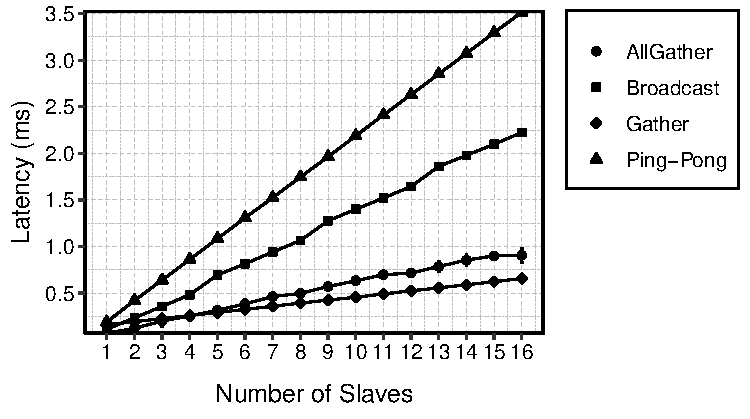
\includegraphics[width=.7\textwidth]{mailbox-latency.pdf}%
			\fonte{Develop by the Author.}%
		\end{figure}
